% \documentclass{beamer}
% \usetheme{Szeged}

% \usepackage{media9}
% \usepackage{graphicx}

% \begin{document}

%-------------------------------------------------------------------------------
%							FOURTH SECTION
%-------------------------------------------------------------------------------
\section{Le problème en 2D}

\subsection{Simulation}

\begin{frame}[fragile]
    \frametitle{Exemple de simulation 2D}
  \begin{center}
    \includemedia[
      width=0.95\linewidth,
      activate=pageopen,
      addresource=Video2D.mp4,
      flashvars={
         source=Video2D.mp4
        &autoPlay=true
      },
      passcontext, % enable VPlayer's right-click menue
    ]{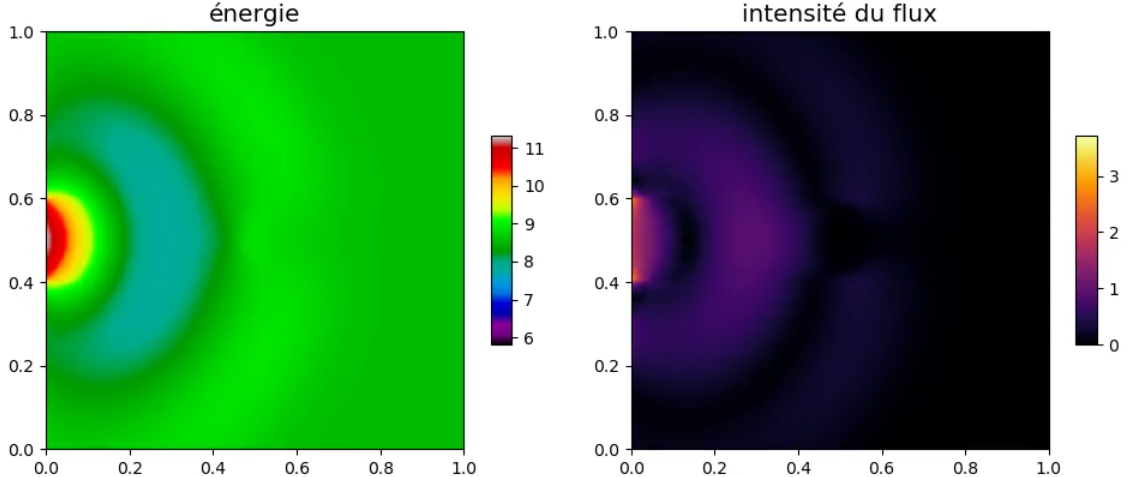
\includegraphics{Thumbnail2D.png}}{VPlayer.swf}%
  \end{center}
\end{frame}

\begin{frame}[fragile]
    \frametitle{Entree sortie 2D}

        \begin{figure}
        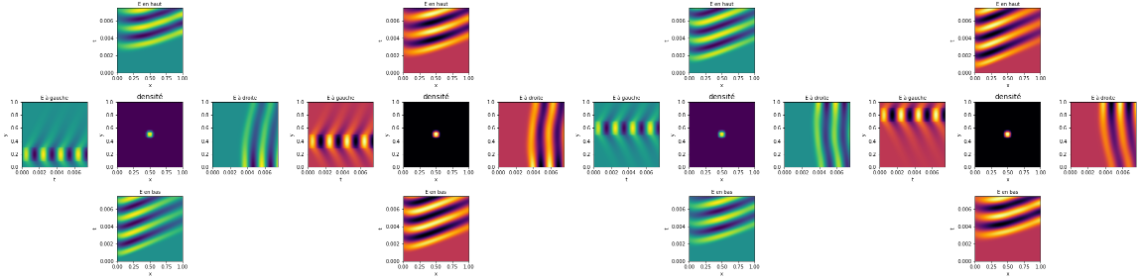
\includegraphics[width=11cm]{EntreeSortie2D}       
        \caption{Entrees sortie pour le reseau de neurones}
        \end{figure}
        \begin{figure}
        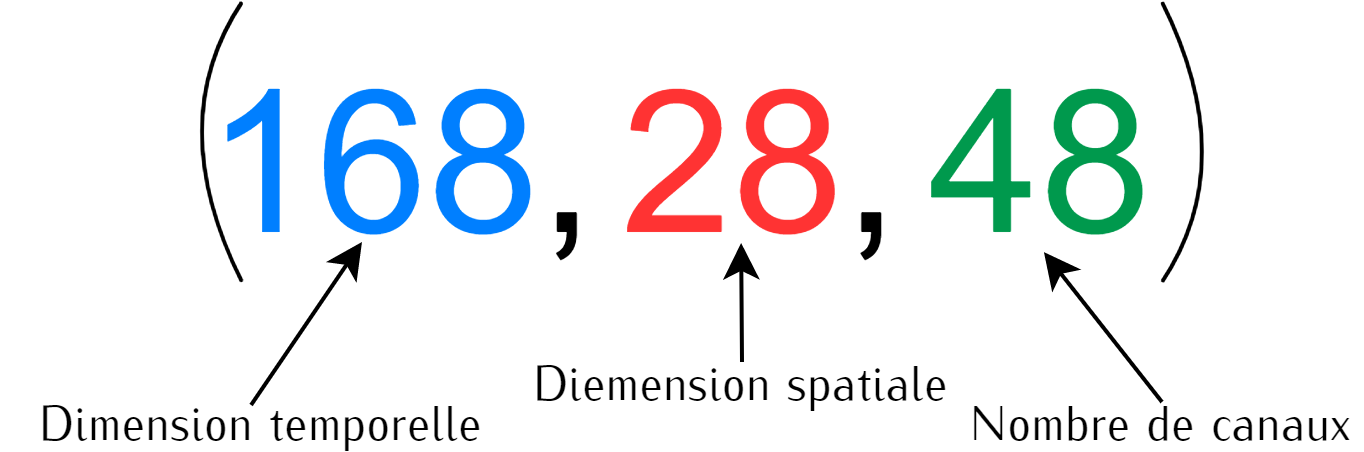
\includegraphics[width=3cm]{Entrees2D}       
        \caption{Taille d'une entree}
        \end{figure}

\end{frame}

\subsection{Apprentissage}

\begin{frame}[fragile]
    \frametitle{Meilleures/pires predictions du reseau de neurones}

    \begin{columns}
    \begin{column}{0.5\textwidth}
        \begin{figure}
        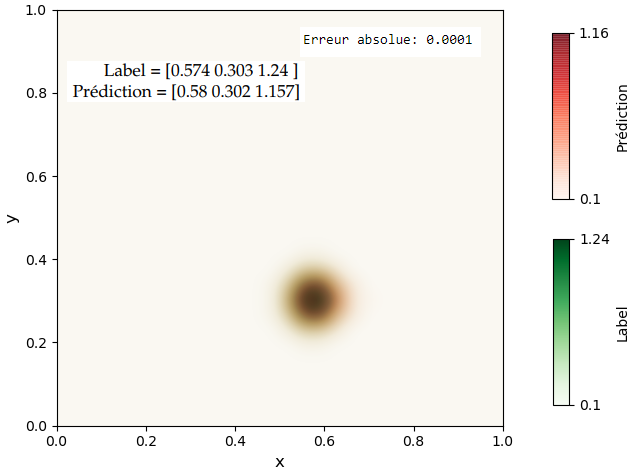
\includegraphics[width=3cm]{Meilleur2D1}       
        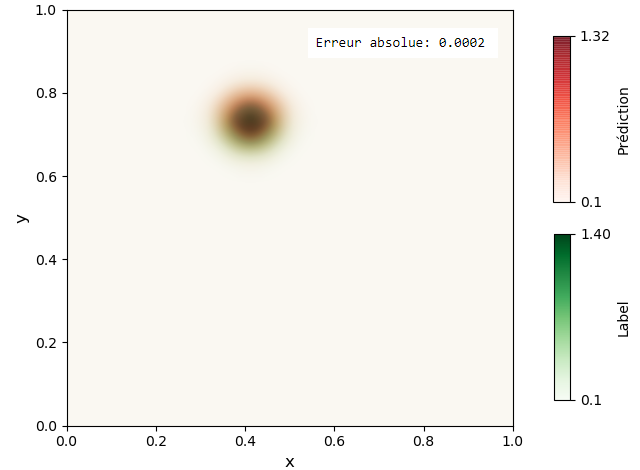
\includegraphics[width=3cm]{Meilleur2D2}       
        \caption{Les meilleures predictions}
        \end{figure}
     \end{column}
     \begin{column}{0.5\textwidth}
        \begin{figure}
        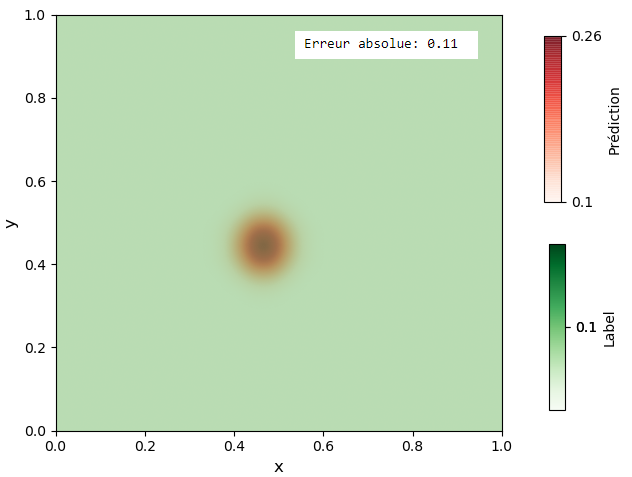
\includegraphics[width=2.5cm]{Pire2D1}       
        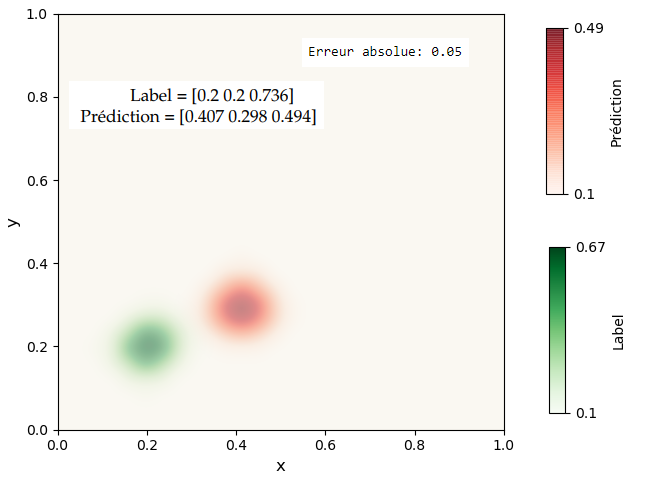
\includegraphics[width=2.5cm]{Pire2D2}       
        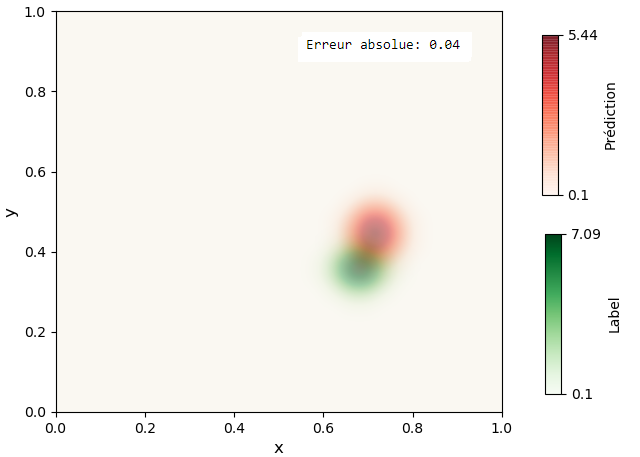
\includegraphics[width=2.5cm]{Pire2D3}       
        \caption{Les pires predictions}
        \end{figure}
     \end{column}
    \end{columns}

\end{frame}

\begin{frame}
    \frametitle{Scores 2D}

    \begin{table}[h!]
        \caption{Scores 2D}
        \centering
        \begin{tabular}{l l}
        \toprule
        \textbf{Nom du score} & \textbf{Valeur} \\
        \midrule
        R2 & 98.81 \%\\
        Personnalisé & 93.50 \%\\
        \bottomrule\\
        \end{tabular}
    \end{table}

    \begin{columns}
        \begin{column}{0.333\textwidth}
            \begin{figure}
            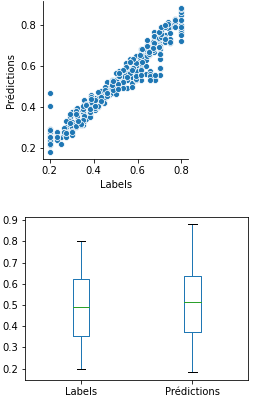
\includegraphics[width=2cm]{PositionX2D}       
            \caption{Correlation de l'abscisse}
            \end{figure}
         \end{column}
         \begin{column}{0.333\textwidth}
            \begin{figure}
            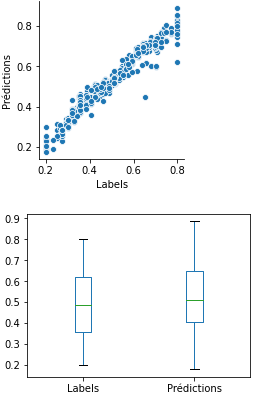
\includegraphics[width=2cm]{PositionY2D}       
            \caption{Correlation de l'ordonee}
            \end{figure}
         \end{column}
         \begin{column}{0.333\textwidth}
            \begin{figure}
            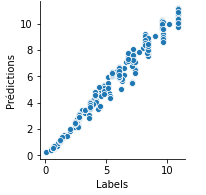
\includegraphics[width=2cm]{Hauteur2D}       
            \caption{Correlation des hauteur}
            \end{figure}
         \end{column}
    \end{columns}

\end{frame}


\begin{frame}
    \frametitle{Conclusion sur la régression 2D}
Detection de toutes les variables:
\begin{itemize}
    \item L'abscisse, l'ordonee, et la hauteur: reconstruction complete de la densite
    \item La valeur de la densite en dehors du crenau est connue
\end{itemize}
\end{frame}

\begin{frame}
    \frametitle{CLassification 2D}
    \begin{columns}
        \begin{column}{0.7\textwidth}
            \begin{figure}
            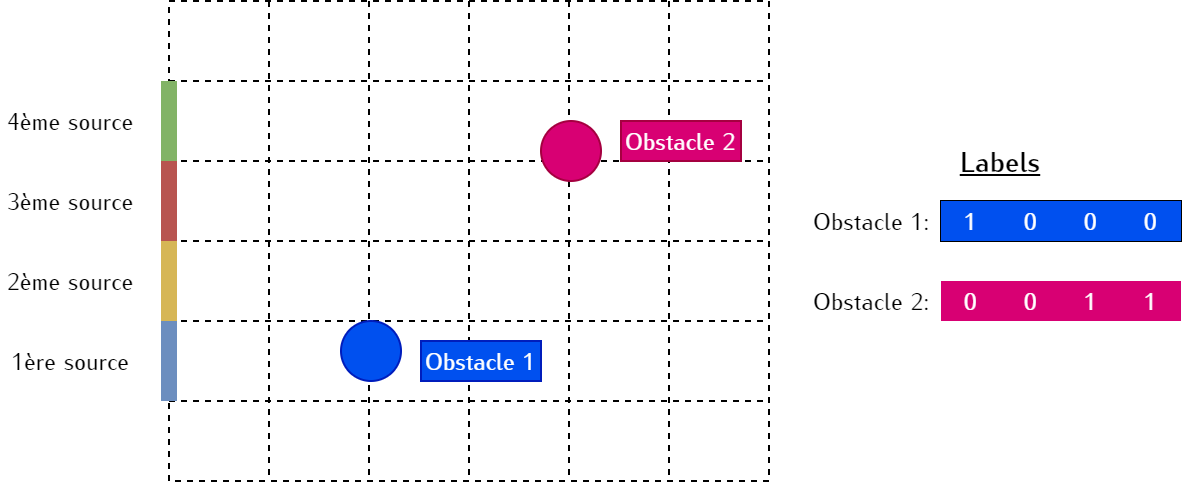
\includegraphics[width=6cm]{Classification}       
            \caption{Labels pour la classification}
            \end{figure}
         \end{column}
         \begin{column}{0.3\textwidth}
            \begin{table}[h!]
                \caption{Scores de classification}
                \centering
                \begin{tabular}{l l}
                \toprule
                \textbf{Nom} & \textbf{Valeur} \\
                \midrule
                R2 & 98.86 \%\\
                Pers. & 95.45 \%\\
                \bottomrule\\
                \end{tabular}
            \end{table}
         \end{column}
    \end{columns}
\end{frame}


% \end{document}
